
%%%% CS553 Cryptography Term Paper TEMPLATE %%%%

%%%% 1. DOCUMENTCLASS %%%%
\documentclass[preprint]{transcrypto}
%%%% NOTES:
% - Change "submission" to "final" for final version
% - Add "spthm" for LNCS-like theorems


%%%% 2. PACKAGES %%%%
\usepackage{lipsum} % Example package -- can be removed
\usepackage[ruled,vlined]{algorithm2e}
\usepackage[T1]{fontenc}
\usepackage{amssymb}
\usepackage{biblatex}
\addbibresource{citations.bib}
% \bibliographystyle{alpha}
\bibliography{abbrev3,crypto}
%%%% 3. AUTHOR, INSTITUTE %%%%
\author{Gagan deep singh(11840480)\inst{1} \and Siram Nikhil\inst{1}(11841090) \and Kolli Madhukar(11840670)\inst{1}}
\institute{
 Indian Institute of Technology, Bhilai, India 
}
%%%% NOTES:
% - We need a city name for indexation purpose, even if it is redundant
%   (eg: University of Atlantis, Atlantis, Atlantis)
% - \inst{} can be omitted if there is a single institute,
%   or exactly one institute per author


%%%% 4. TITLE %%%%
\title{KLIEN CIPHER}
%%%% NOTES:
% - If the title is too long, or includes special macro, please
%   provide a "running title" as optional argument: \title[Short]{Long}
% - You can provide an optional subtitle with \subtitle.

\begin{document}

\maketitle


%%%% 5. KEYWORDS %%%%
\keywords{Block Cipher \and Low Resource Implementation \and  Ubiquitous computing. }
%%%% 6. ABSTRACT %%%%
\begin{abstract}
In the day to day life, the usage of IoT is increasing exponentially.Parallely the need of the security will also increase as the user base of Ubiquitous computing increases. As most of the IoT applications involve the usage of low end devices like sensors, RFIDs etc the security algorithms should be suitable the resources available to them. KLEIN is one of the lightweight cipher which is designed mainly for sensors. In Section 1, the need of lightweight cipher like KLEIN is described.In Section 2 and 3 design decisions and specification the KLEIN cipher are mentioned. Before wide implementation of any cipher, a good amount of time should be spent doing cryptanalysis on it. In Section 4, various attacks like Differential analysis, Round reduced analysis and Integral cryptanalysis is done.
\end{abstract}


%%%% 7. PAPER CONTENT %%%%
\section{Introduction}
As the development and usage of wireless computing and embedded systems is increasing we are being increasingly dependent on Ubiquitous computing examples are sensors, RFID tags etc. On these limited resource systems the selection of the security algorithms must be done carefully by taking the implementation costs along with the level of security provided. So the Era of light-weight cryptography is started. Many algorithms with various design strategies were proposed.Few of them were skipjack, KATAN\cite{KATAN}, KTANTAN\cite{KATAN}, PRESENT\cite{PRESENT} etc. skipjack is 8 bit key and 64-bit block length cipher whose basic design is based on unbalanced feistal network. PRESENT is 80/128 bit key and 64 bit block size cipher  which is extremely hardware efficient as the diffusion layer constitutes of only wiring with no algebraic unit.
Before wide implementation of a security algorithm, it should be thoroughly analysed. As the result of these analysis an attack on 31 out of 32 rounds of skipjack based on impossible differential is discovered. Also there are weak key attacks and linear attacks on PRESENT.Hence the need of secure lightweight-ciphers did not came to and end. KLEIN is a lightweight block cipher which is mainly invented for devices like sensors which have very less resources. KLEIN \cite{KLEIN} is based on Substitution Permutation Networks. In this paper we will be seeing the working of KLEIN cipher, implementation details and different attacks performed on it along with the comparison of performance and security among few other .
\section{Design rationale}
In this section we will be discussing about design rationale chosen when creating KLEIN ciphers.
\\
KLEIN is collection of ciphers of different key length(64, 80, and 96) and fixed 64 bit block length.
We shall denote these ciphers as KLEIN-64/80/96 based on their key lengths.We know that block cipher's security and implementation cost mainly depends on the key size and block size. Keeping in mind that lightweight ciphers are used in resource constrained machines like sensors, RFIDs, the block length is decided to be 64 bits as high-throughput is not expected in these devices as large block lengths and larger keys are unnecessary. As 64 bit key length might be little vulnerable if we consider attacks based on pre-computation and large storage capacities, it is suggested to use KLEIN-64 for message authentication codes and hash functions, Where as KLEIN-80/96 are to be used for encryption in any of the modes of operation.

\subsection{Optimal Platform} Generally light weight ciphers are optimized for hardware implementation as they are used in RFID tags and smart cards. But if a system can support the computation and memory requirements of the software implementation, the costs of manufacturing and maintenance will reduce drastically as we can simply update the implementation of the cipher by simply installing a software update. They are also more flexible. So they mainly focused on the software implementation of KLEIN. 
But both the software and hardware implementations are light weight.
\subsection{Critical Threats}
At the basic, the cipher should be resistant to general attacks like differential and linear. An for a cipher to be secure enough and implemented widely it should also be resistant to the related key attacks and the ones which belong to Grey box model like side channel attacks. Even if the sensor nodes are compromised they should not be able to crack the cipher. But generally the hardware implementations are vulnerable to the side channel attacks like differential power analysis etc. The protection methods of these side channel attacks like Blindfolding, making and re-keying techniques are suitable enough for normal ciphers in terms implementation costs. For lightweight ciphers their costs should as minimal as possible. The Key schedule of KLEIN is said to balanced enough as it is resistant against related key attacks. 

\section{Specification of KLEIN}

\subsection{Structure of KLEIN}
KLEIN is made of Substitution-Permutation-Network(SPN) which is also used in popular ciphers like AES and PRESENT. By taking into the consideration of security margin and the asymmetric iteration we chose 12/16/20 rounds for KLIEN-64/80/96 respectively. $N_{R}$ is used to represent the number of rounds.\\
The pseudo-code of KLEIN is displayed below.\\

\begin{algorithm}[H]
\SetAlgoLined
$sk^{1}\gets KEY$; \\
STATE $\gets$ PLAINTEXT;\\
\For{$i=1$ \KwTo $N_{R}$ }{
    $AddRoundKey(\text{STATE}, sk i );$\\
$SubN ibbles(\text{STATE});$ \\
$RotateN ibbles(\text{STATE});$ \\
$MixN ibbles(\text{STATE});$ \\
$sk_{i+1} = KeySchedule(sk_{i} , i);$ \\
 }
 CIPHERTEXT $\gets AddRoundKey(\text{STATE}, sk^{N_{R}+1} )$;
 \caption{KLEIN CIPHER}
\end{algorithm}
\subsection{Round Transformation}
The Input and Out put of KLEIN is in terms of one-dimensional array of bytes. All the steps in each round can be optimized by byte-oriented algorithms. \textbf{Image should be added here}.
\subsubsection{SubNibbles step}
Before this step, the corresponding round key will be xor-ed with the input . The obtained resultant state is passed to subnibbles where the state is divided into 16 4-bit nibbles and given as input to the 4 x 4 Involutive permutation. Involutiveness of S-box is helpful to decrease the implementation costs of calculating its inverse and also the need of protect only one sbox instead of two(original and inverse) in other ciphers from side channel attacks.
\begin{center}\begin{math}
\begin{array}{|c|c|c|c|c|c|c|c|c|c|c|c|c|c|c|c|c|}
\hline
Input &0 &1 &2 &3 &4 &5 &6 &7 &8 &9 &A &B &C & D& E& F&  
\hline
Output &7 &4 &A &9 &1 &F &B &0 &C &3 &2 &6 &8 &E &D &5 & 
\hline
\end{array}
\end{math}
\end{center}
To obtain the required resistance against linear and differential cryptanalysis, The Sbox should have this properties:
\begin{enumerate}
    \item It satisfies $S(S(x)) = x, x \in \mathbb{F}^{4}_{2} $, as it is said to be Involutive.
    \item  It should not contain any fixed points i.e S(x)$\neq$x, where  $x \in \mathbb{F}^{4}_{2} $.
    \item For any non-zero input diff($\Delta_{I}$) and output diff($\Delta_{O}$) that belong to  $\mathbb{F}^{4}_{2} $, It should follow:
    $$ \#\{x \in \mathbb{F}^{4}_{2} | S(x) \oplus S(x \oplus \Delta_{I} ) = \Delta_{O} \} \leq 4$$.
    Furthermore, if $wt(\Delta_{I} ) = wt(\Delta{O} )=1$, where $wt(X)=\sum_{i}X_{i}\;$($X_{i}$ is ith bit of X) , we have
$$\#\{x \in \mathbb{F}^{4}_{2} |S(x) \oplus S(x \oplus \Delta_{I} ) = \Delta_{O} \} \leq 2$$.
\end{enumerate}



\subsubsection{Rotate Nibbles step}

Assume at the ith round state is $ b_{0} b_{1} b_{2} b_{3} b_{4} b_{5} b_{6} b_{7} b_{8} b_{9} b_{10} b_{11} b_{12} b_{13} b_{14} b_{15} $ where $b_{i}$ is a nibble. The rotate nibble step involves left circular shift of two bytes of this state i.e after the rotate nibbles step our state becomes $   b_{4} b_{5} b_{6} b_{7} b_{8} b_{9} b_{10} b_{11} b_{12} b_{13} b_{14} b_{15} b_{0} b_{1} b_{2} b_{3} $ 

\subsubsection{Mix nibbles step}
Let the current state be $c_{0} c_{1} c_{2} c_{3} c_{4} c_{5} c_{6} c_{7} c_{8} c_{9} c_{10} c_{11} c_{12} c_{13} c_{14} c_{15}$\\
Now first this state is divided into two parts \\
$ c_{0} c_{1} c_{2} c_{3} c_{4} c_{5} c_{6} c_{7} $ and $c_{8} c_{9} c_{10} c_{11} c_{12} c_{13} c_{14} c_{15}$ \\
We denote each of this part as a single column matrix with each element as 8-bit($c_{i}|c_{i+1}$) \\. The next state in the algorithm is obtained by multiplying(details needed ) this columns with a fixed matrix.This alogorithm is same as the MixColumns step in AES(Rijndael).All the steps in the round function are nibble wise operation except MixColumns which is byte wise. This operation is performed in GF(8) with modulo polynomial as $x^{8} + x^{4} + x^{3} + x + 1$.\\ \\
$\begin{bmatrix}
s^{i+1}_{0} | s^{i+1}_{1}\\
s^{i+1}_{2} | s^{i+1}_{3}\\
s^{i+1}_{4} | s^{i+1}_{5}\\
s^{i+1}_{6} | s^{i+1}_{7}
\end{bmatrix}=
\begin{bmatrix}
2&3&1&1\\
1&2&3&1\\
1&1&2&3\\
3&1&1&2
\end{bmatrix}
\begin{bmatrix}
c_{0}|c_{1}\\
c_{2}|c_{3}\\
c_{4}|c_{5}\\
c_{6}|c_{7}
\end{bmatrix}  $ ,
$\begin{bmatrix}
s^{i+1}_{8} | s^{i+1}_{9}\\
s^{i+1}_{10} | s^{i+1}_{11}\\
s^{i+1}_{12} | s^{i+1}_{13}\\
s^{i+1}_{14} | s^{i+1}_{15}
\end{bmatrix}=
\begin{bmatrix}
2&3&1&1\\
1&2&3&1\\
1&1&2&3\\
3&1&1&2
\end{bmatrix}
\begin{bmatrix}
c_{8}|c_{9}\\
c_{10}|c_{11}\\
c_{12}|c_{13}\\
c_{14}|c_{15}
\end{bmatrix}  $\\ \\
Thus we obtain the next state 
$ s^{i+1}_{0}  s^{i+1}_{1}
s^{i+1}_{2}  s^{i+1}_{3}
s^{i+1}_{4}  s^{i+1}_{5}
s^{i+1}_{6}  s^{i+1}_{7}
s^{i+1}_{8}  s^{i+1}_{9}
s^{i+1}_{10}  s^{i+1}_{11}
s^{i+1}_{12}  s^{i+1}_{13}
s^{i+1}_{14}  s^{i+1}_{15} $


\subsubsection{Key Schedule}
We call the original key as master key and denote it as $mk$. It will be of 64/80/96 bit for  KLIEN 64/80/96. As a result of key scheduling algorthm 8/10/12  subkeys with length same as master key will be generated for KLIEN 64/80/96. Without LOG we will talk about key scheduling of KLEIN 64 \\

\begin{itemize}

\item The first subkey $sk_{0}$ is same as the master key \\
	$sk_{0}$=$mk$.Each of the subsequent $sk_{i+1}$ will be derived from $sk_{i}$ as follows - 

\item Denote $sk_{i}$ as a tuple of bytes - (x0 x1 x2 x3 x4 x5 x6 x7) \\
Divide the tuple into two equal parts and call them a and b 

a - ($ x_{0}$ $x_{1}$ $x_{2}$ $x_{3}$) \\
b - ($x_{4}$ $x_{5}$ $x_{6}$ $x_{7}$) 

\item Now Perform one byte left circular shift to both a and b

$a'$ = ($x_{1}$ $x_{2}$ $x_{3}$ $x_{0}$) \\
$b'$  = ($x_{7}$ $x_{4}$ $x_{5}$ $x_{6}$) \\

\item Swap $a'$ and $b'$  i.e $a''$ = $b'$  and b''=$a'$ \\

\item Now let $a''$ = ($y_{0}$ $y_{1}$ $y_{2}$ $y_{3}$) \\
and $b''$ = ($z_{0}$ $z_{1}$ $z_{2}$ $z_{3}$) \\

We will Xor the round counter i with 3rd byte of $a''$ and pass 2nd and 3rd byte of $b''$ through the KLIEN S-BOX and then $a''$|$b''$ will become the next subkey \\
$sk_{i+1}$ = (y0 y1 $ y2 \oplus R_i $ y3 z0 Sbox(z1) Sbox(z2) z4)
\end{itemize}

\begin{figure}[h!]
    \centering
    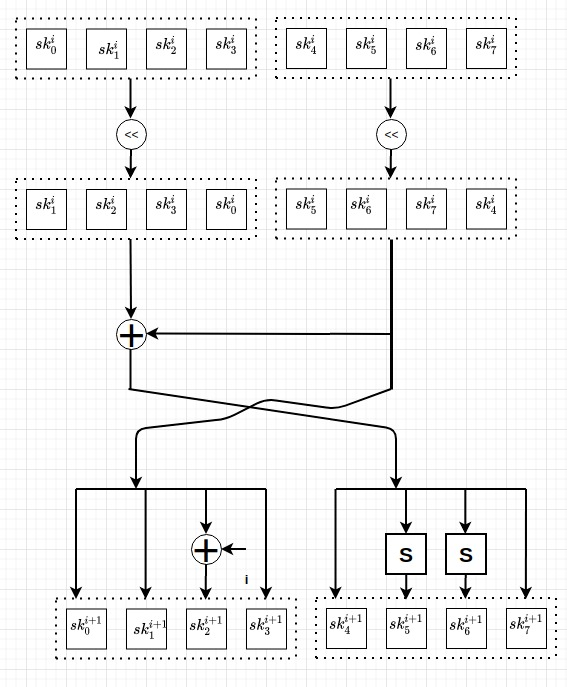
\includegraphics[width=8cm, hieght= 10cm, keepaspectratio]{images/key_schedule.jpeg}
    \caption{Key Schedule}
    \label{fig:key schedule}
\end{figure}


    \begin{figure}[h!]
    \centering
    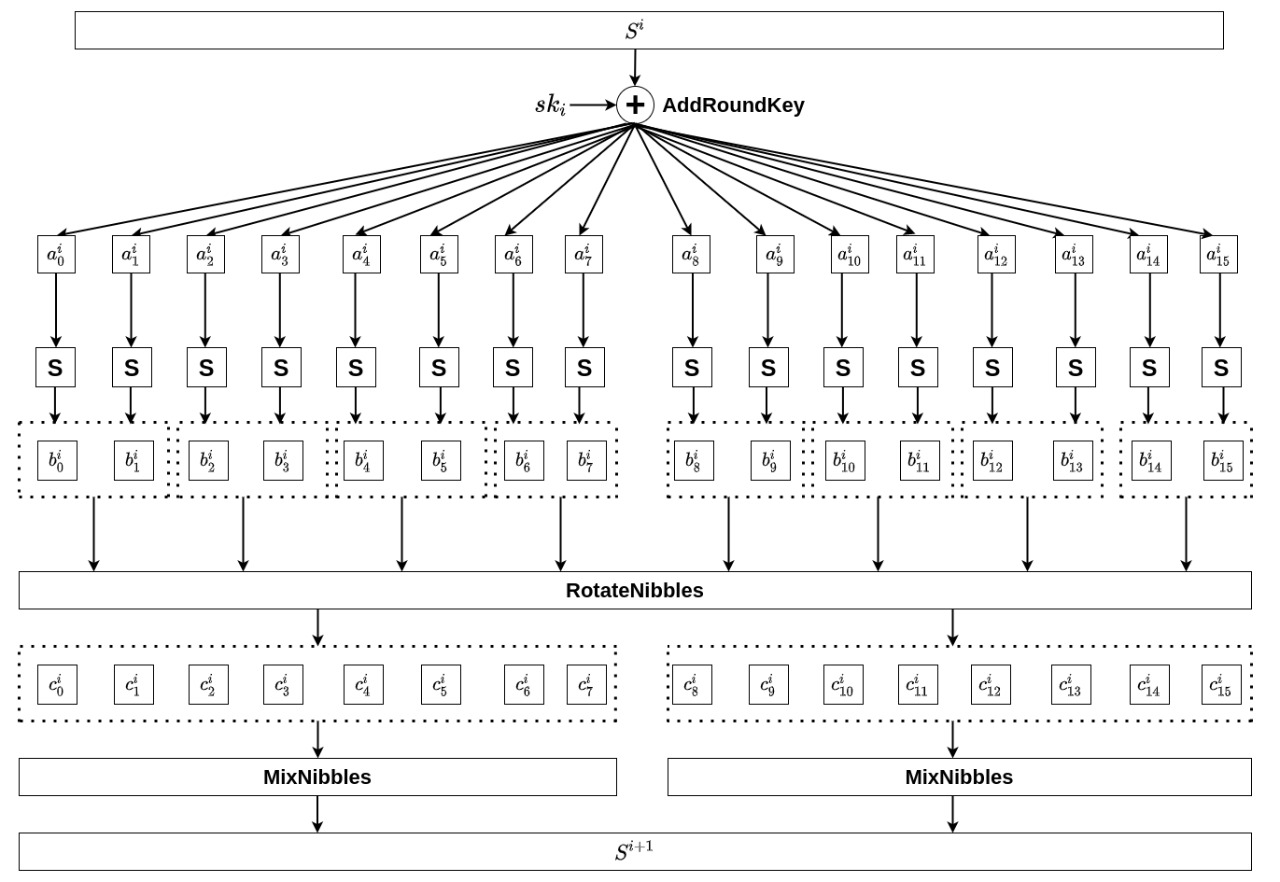
\includegraphics[width= \textwidth]{images/klein_cipher.jpeg}
    \caption{KLEIN cipher}
    \label{fig:overview}
\end{figure}


\section{Various Attacks on KLEIN}
Before we proceed to the analysis of attacks done on KLEIN, let us analyze some properties of SBOX.\\
The DDT(Differential Distribution Table) of SBOX is written below:
\begin{center}
\begin{tabular}{|c|c|c|c|c|c|c|c|c|c|c|c|c|c|c|c|c|}
\hline
$\Delta_{In}|\Delta_{Out}$ &0&1&2&3&4&5&6&7&8&9&10&11&12&13&14&15 \\
\hline
0&16& 0& 0& 0& 0& 0& 0& 0& 0& 0& 0& 0& 0& 0& 0& 0 \\
\hline
1&0& 0& 0& 4& 2& 0& 2& 0& 2& 0& 0& 2& 0& 0& 2& 2 \\
\hline
2&0& 0& 0& 0& 0& 4& 0& 0& 0& 0& 2& 2& 0& 4& 2& 2 \\
\hline
3&0& 4& 0& 2& 2& 0& 0& 0& 0& 0& 2& 0& 0& 2& 4& 0 \\
\hline
4&0& 2& 0& 2& 2& 0& 2& 0& 0& 2& 0& 2& 0& 2& 0& 2 \\
\hline
5&0& 0& 4& 0& 0& 2& 0& 2& 2& 0& 2& 4& 0& 0& 0& 0 \\
\hline
6&0& 2& 0& 0& 2& 0& 4& 0& 2& 0& 2& 2& 2& 0& 0& 0 \\
\hline
7&0& 0& 0& 0& 0& 2& 0& 2& 2& 2& 0& 0& 2& 0& 4& 2 \\
\hline
8&0& 2& 0& 0& 0& 2& 2& 2& 2& 2& 0& 2& 0& 0& 0& 2 \\
\hline
9&0& 0& 0& 0& 2& 0& 0& 2& 2& 0& 0& 2& 2& 2& 2& 2 \\
\hline
10&0& 0& 2& 2& 0& 2& 2& 0& 0& 0& 4& 0& 2& 0& 2& 0 \\
\hline
11&0& 2& 2& 0& 2& 4& 2& 0& 2& 2& 0& 0& 0& 0& 0& 0 \\
\hline
12&0& 0& 0& 0& 0& 0& 2& 2& 0& 2& 2& 0& 4& 2& 0& 2 \\
\hline
13&0& 0& 4& 2& 2& 0& 0& 0& 0& 2& 0& 0& 2& 2& 0& 2 \\
\hline
14&0& 2& 2& 4& 0& 0& 0& 4& 0& 2& 2& 0& 0& 0& 0& 0 \\
\hline
15&0& 2& 2& 0& 2& 0& 0& 2& 2& 2& 0& 0& 2& 2& 0& 0 \\
\hline
\end{tabular}
\end{center}
The maximum differential probability is KLEIN's SBOX is 4/16 i.e 1/4 and some of the transitions leading to it are $(\Delta_{In},\Delta_{Out})$= (1,4),(3,1) etc.\\
If we the input to sbox can be represented as $x=x_{0}||x_{1}||x_{2}||x_{3}$ and the output is represented as $y = y_{0}||y_{1}||y_{2}||y_{3}$, then the ANF represnatio of KLEIN's SBOX is given as :\\

\begin{math}
y_{0} = 1+ x_{0} + x_{1} + x_{3} + x_{0} x_{2} + x_{1} x_{2} + x_{1} x_{3}+ x_{0}x_{1}x_{2}+  x_{0}x_{1}x_{3}\\
y_{1}= 1+ x_{0}+ x_{2}+ x_{3}+ x_{1}x_{2}+ x_{1}x_{3}+ x_{2}x_{3}+ x_{0}x_{1}x_{3} \\
y_{2}= 1+ x_{1}+ x_{2}+ x_{0}x_{2}+ x_{1}x_{2}+ x_{0}x_{3}+ x_{0}x_{1}x_{2}+ x_{0}x_{2}x_{3}+ x_{1}x_{2}x_{3}\\
y_{3} = x_{1}+ x_{3}+ x_{0}x_{2}+ x_{0}x_{3}+ x_{0}x_{1}x_{3}+ x_{1}x_{2}x_{3} \\
\end{math}


\subsection{Cryptanalysis of Reduced-Round KLEIN Block Cipher} \cite{reduced_round}
The weakness present in the Rotate Nibbles and Mix columns step is exploited here in this attack.\\
Firstly, a 6 round truncated differential distinguisher with $2^{-29}$ is made.Using this as base, an 8 Round distinguisher is constructed.One of the assumption is they will be having access to round wise outputs.\\
Lets have look at few terminologies used in this attack:\\
\begin{enumerate}
    \item $X_{i}$ : The input of the i-th round.
    \item $\Delta X_{i}$ : The input difference of the i-th round.
    \item $Y_{i}$ : The input of SubNibbles in the i-th round .
    \item $\Delta Y_{i}$ : The input difference of SubNibbles in the i-th round .
    \item $X_{i,j}$ : The j-th nibble of the $X_{i}$ , where j = 0, 1, ...15.
    \item $sk_{i}$ : The subkey of the i-th round.
    \item $X || Y$ : The the concatenation of X and Y.
\end{enumerate}
The state of encryption: \\
\begin{center}
\begin{tabular}{|c|c|c|c|}
\hline
0&4&8&12\\
\hline
1&5&9&13\\
\hline
2&6&10&14 \\
\hline
3&7&11&15\\  
\hline
\end{tabular}
\end{center}
The number in box represents the Nibble numbers of the 64 bit data block.


\subsubsection{Truncated Six Round Differential Distinguisher}
As it is based the limitations of MixColumns and RotateNibbles, few properties and observations are listed.\\
\textbf{Property 1} As the mix columns operation is same as the one used in Rijndael. We know that the multiplication is done in $GF(8)$ using modulo polynomial m(x)= $x^{8} + x^{4} + x^{3} + x + 1$.\\
Take a polynomial in $GF(8)$ of the form $f(x) = b^{7} x_{7} + b^{6} x_{6} + b^{5} x_{5} + b^{4} x_{4} + b^{3} x_{3} + b^{2} x_{2} + b^{1} x + b^{0}$.\\
Result of multiplication of $x$ to $f(x)$ is\\
$$x * f(x) = (b_{6} b_{5} b_{4} b_{3} b_{2} b_{1} b_{0} 0)\;\; \text{if}\,b_{7}=0$$ 
$$ x * f(x) = (b_{6} b_{5} b_{4} b_{3} b_{2} b_{1} b_{0} 0) \oplus (00011011) \;\; \text{if} b_{7} = 1$$ 
\textbf{Lemma1.} If a byte is of the form $0z$, where $z$ is a 4-bit string
with MSB bit as 0, then $0z$ multiply by $x$ is equal to $0z^{'}$, where $z ^{'}$
is a 4-bit string.\\
The following observations are derived based on above lemma.\\ \\
\textbf{Observation 1.} 
\begin{math}
\begin{bmatrix}
2&3&1&1\\
1&2&3&1\\
1&1&2&3\\
3&1&1&2
\end{bmatrix}
\text{x}
\begin{bmatrix}
0z \\
00 \\
00 \\
00 
\end{bmatrix} = 
\begin{bmatrix}
0z^{'}_{1} \\
0z^{'}_{2} \\
0z^{'}_{3} \\
0z^{'}_{4} 
\end{bmatrix}
\end{math} if only if MSB $z$ is 0. \\ \\
Observation 1 holds with the probability $2^{-1}$, because the only requirement is that the MSB of $z$ must be 0 and the probability of this event to occur is 1/2.\\ \\
\textbf{Observation 2.} 
\begin{math}
\begin{bmatrix}
2&3&1&1\\
1&2&3&1\\
1&1&2&3\\
3&1&1&2
\end{bmatrix}
\text{x}
\begin{bmatrix}
00 \\
00 \\
0z_{1} \\
0z_{2} 
\end{bmatrix} = 
\begin{bmatrix}
0z^{'}_{1} \\
0z^{'}_{2} \\
0z^{'}_{3} \\
0z^{'}_{4} 
\end{bmatrix}
\end{math} if only if MSB $z_{1}$ and $z_{2}$ is 0. \\ \\
Observation 2 holds with the probability $2-2$, because the requirement is that the MSB of $z_{1}$ and $z_{2}$ must be 0 and the probability of this event to occur is (1/2)*(1/2). The reason for this requirment is statete below.\\ \\
\textbf{Reason}: 
\begin{math}
\begin{bmatrix}
2&3&1&1\\
1&2&3&1\\
1&1&2&3\\
3&1&1&2
\end{bmatrix}
\text{x}
\begin{bmatrix}
00 \\
00 \\
0z_{1} \\
0z_{2} 
\end{bmatrix} = 
\begin{bmatrix}
(0z_{1}) \oplus (0z_{2})\\
3(0z_{1}) \oplus (0z_{2}) \\
2(0z_{1}) \oplus 3(0z_{2})) \\
(0z_{1}) \oplus 2(0z_{2}))
\end{bmatrix}
\end{math}\\ \\ \\
for $3(0z_{1}) \oplus (0z_{2})\,,\,2(0z_{1}) \oplus 3(0z_{2}))\; and\; (0z_{1}) \oplus 2(0z_{2}))$ to be of the form $0z$, the MSB's of $z_{1}$ and $z_{2}$ should be equal to 0 according to Lemma1.
\\ \\
\textbf{Observation 3}
\begin{math}
\begin{bmatrix}
2&3&1&1\\
1&2&3&1\\
1&1&2&3\\
3&1&1&2
\end{bmatrix}
\text{x}
\begin{bmatrix}
0z_{1} \\
0z_{2} \\
0z_{3} \\
0z_{4} 
\end{bmatrix} = 
\begin{bmatrix}
0z^{'}_{1} \\
0z^{'}_{2} \\
0z^{'}_{3} \\
0z^{'}_{4} 
\end{bmatrix}
\end{math}
 if only if MSB's of $z_{1},
z_{2} ,
z_{3} \;and\;
z_{4} $ are 0.\\
The probability of the above requirement is $2^{-2}$. The proof will be similar to the above reason in observation 2.\\
\\Based on the above observations, we show that if the input difference of 6-round KLEIN are all zero except the 13-th nibble, after encryption, the first and the third column of state matrix will
stay 0 with the probability of $2^{-29}$.\\
This happens because the difference in column will not transfer to other column due to the RotateBits algorithm and above observations. \\ This is the reason for high probability 6-round differential distinguisher.

\subsubsection{Truncated Differential Analysis of 8-Round KLEIN-64}
The 8 round distinguisher is constructed by adding an extra layer at the top and bottom of the 6 round distinguisher.\\
As this is CPA(chosen plain text) attack, we choose plain text pairs such a way that input difference to the second round is all zero except the 13-th nibble. We actually obtain the required input pairs of first round by reverse tracing the single nibble that should be active at the end of the round.This process is also diplayed in Figure \ref{fig:8distinguisher} \\

\begin{center}
\begin{math}
MC^{-1} *  
\begin{bmatrix}
00 \\
00 \\
01 \\
00
\end{bmatrix}
=
\begin{bmatrix}
0d \\
0b \\
0e \\
09
\end{bmatrix}
\end{math}    
\end{center}
This is the state of last column that we require after the Rotate bits.The further structure of the first Round is shown in Figure \ref{fig:6distinguisher}.
\begin{figure}[h!]
    \centering
    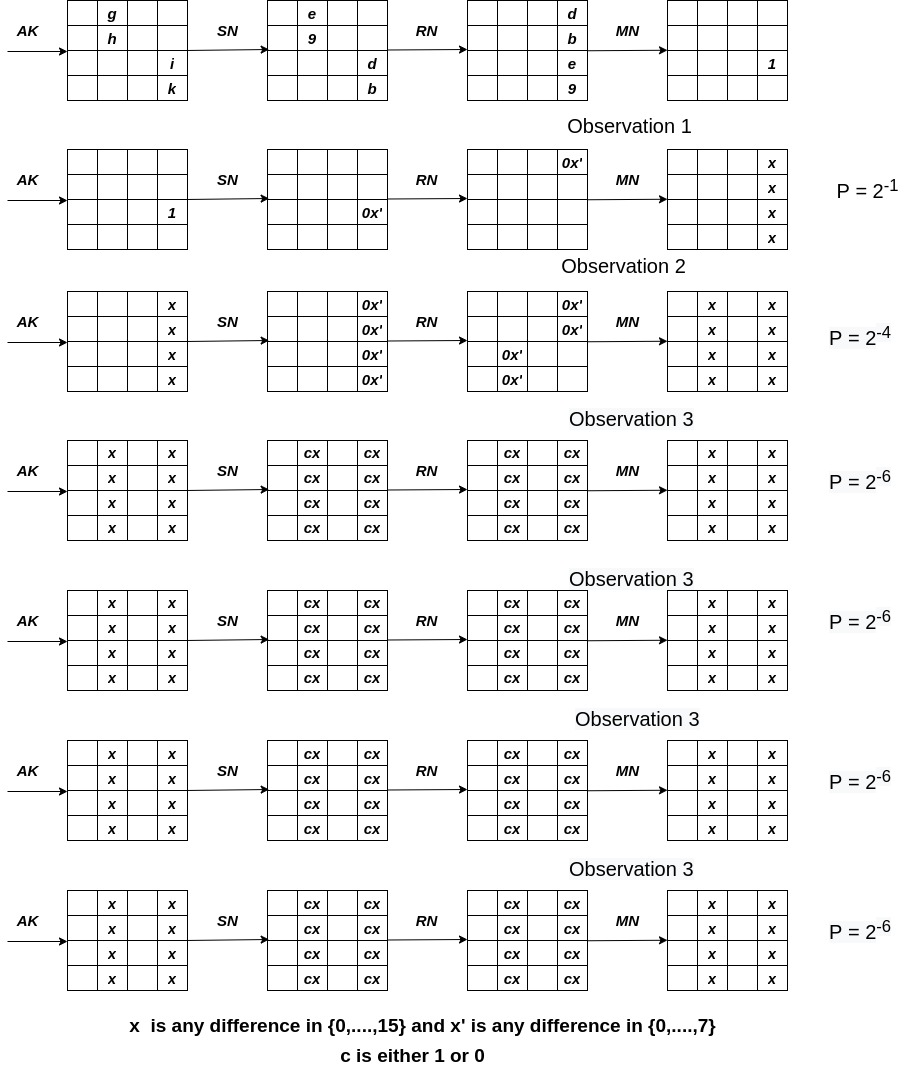
\includegraphics[width= \textwidth]{images/7round characteristic of round reduced.jpg}
    \caption{7 round characteristic of 8 Round Distinguisher}
    \label{fig:6distinguisher}
\end{figure}
\\ \\
\textbf{ The Steps and Analysis Procedure}\\ \\
\begin{enumerate}
\item We will choose the input plaintexts in such a way that, all nibbles have some fixed values except four nibbles $X_{1,1} , X_{1,3} , X_{1,13} , X_{1,15}$. If we fix the values and change the values only in these 4 nibbles, that is called one structure. There are $2^{16}$ possible plain texts in one structure.
We can form nC2 i.e $(2^{16} \text{x} (2^{16} - 1))/2 = 2^{31}$ plain text pairs from those $2^{16} $ plain texts.\\ If we took m structures then we will have $2^{16}m$ plain texts and $2^{31}m$ pairs.\\
\item By Guessing the values(trying all possible values)  of the subkey nibbles $sk_{1,1} , sk_{1,3} , sk_{1,13} , sk_{1,15}$ we should make sure that $\Delta SubNibbles(X_{1,1} \oplus sk_{1,1} ) = 0e, \Delta SubNibbles(X_{1,3} \oplus sk_{1,3} ) = 09, \Delta SubNibbles(X_{1,13} \oplus sk_{1,13} ) =
0d\; and \;\Delta S(X_{1,15} \oplus sk_{1,15} ) = 0b.$ The probability of this is $2^{-16}$ as we are fixing values of 4 particular nibbles, so the expected number of confirming pairs is $2^{31} \;\text{x}\; m\; \text{x} \;2^{-16} = 2^{15} m$. \\
\item  Now take those remaining $2^{15}m$ pairs and encrypt them upto 8 rounds. Then verify the third and first columns output difference of $MC^{-1}$  to zero. If not, discard the key guess. The probability of this event to happen is $(2 ^{-16})^{2}$ so the number of confirming pairs would be $2^{15} \;*\; m \;*\; (2 ^{-16})^{2} = 2^{-17}m$. Now we should use meet in the middle technique. \\ 
\item  For the obtained confirming pairs from previous step,  guess the value of the subkey $sk_{9,j}$, j = 0, 1, \ldots, 7 to inverse the SubNibbles step and find input difference of 8-th round, i.e $\Delta X_{8,j}$ , j = 0, 1, \ldots, 7. \\
\item Now, reverse the MixColumns step i.e $MC^{-1}$ on $\Delta X_{8}$ and verify whether the first column difference is zero and also the MSB of second column should be all 1 or all 0. If it failed to satisfy the above condition then discard the key guess.The expected confirming pairs is $2^{17}\;*\;m\;*\;2^{-7} = 2^{-24}m$ as the probability of the above event is $2^{-7}$.
\item Guess the remaining 16 bits key in the similar way by verifying third and fourth columns.

\end{enumerate}
\textbf{Success Probability and Complexity} \\ \\
All the above analysis is for calculating probability for any random pair of plain text pair confirming the differential with a random key.\\
So the the no.of plaintext pairs that become a confirming pairs under a wrong key are $2^{-24}\,*\,2^{16} = 2^{-8}$ if m=$2^{16}$.\\
The no.of plain text pairs that become a confirming pair under a correct key are $2^{15}\,*\,2^{16}\,*\,2^{-29} = 2^{2}$ for m=$2^{16}$, as the probability of truncated differential is $2^{-29}$.\\ 
\textbf{Time and Space Complexity} \\
Step 2 takes $2^{16}*2^{16}/8$ one round 64 bit encryptions. In Step 3 it takes $2^{15}*2^{16}*2^{16}*7/8$ encryptions whereas in step 4 it takes $2^{-17}*2^{16}*2^{16}*2^{32}/8$ encryptions are required and step 6 takes about $2^{16}$ encryptions.So overall time complexity $2^{46.8}$ one round 64 bit encryptions.The data complexity is $2^{32}$ plaintexts. Memory complexity is $2^{32}$ 64bit states. 

% Gagan


\subsection{Integral Cryptanalysis}

Assume n plaintexts are chosen.We define the following 

1.A nibble is said to be \textbf{Balanced} if the sum of its output across all inputs is 0

2.A nibble is said to be \textbf{Active} if it attains all the possible input values 

\subsubsection{5 round integral distinguisher}

\textbf{Observations}\\ \\

(1) If we give $2^{32}$ different input values to the Rotate Nibble then after the Rotate Nibble and sub nibble operation and 3 rounds of KLIEN all the output nibbles are balanced \\ \\

(2) If in the input state $i_{th}$ nibble is active where i=0,1,2,3,12,13,14,15 then after 1 round of KLIEN and one add key and one sub nibble all $j_{th}$ nibbles are active where j=8,9,10,11,12,13,14,15\\ \\
One more consequence of Observation 2 is that if we give $2^{32}$ different input values with $i_{th}$ nibble  active where i=0,1,2,3,12,13,14,15 then after 1 round of KLIEN and one add key and one sub nibble we will also get $2^32$ different values as 8 active . Now when this output goes into rotate nibble using observation 1 we get all Balanced nibbles after a Rotate Nibble and 3 rounds of KLIEN.\\ \\
So we can state the following proposition now 
\\ \\
If we chose $2^{32}$ different plaintext such that (i) All plaintexts are unique and (ii) The ith nibble is active where i=0,1,2,3,12,13,14,15  then after 5 rounds of KLIEN encryption all the nibbles come out as balanced(i.e their output sum is 0)\\ \vspace{0.1\linewidth}\\
\begin{tabular}{|c|c|c|c|c|c|c|c|}
	\hline
	A & A & C & A & C & C & C & C \\
	\hline
	C & C & C & C & A & A & A & A\\
	\hline
\end{tabular}
$\xrightarrow{1.5round}$
\begin{tabular}{|c|c|c|c|c|c|c|c|}
	\hline
	X & X & X & A & X & X & X & X \\
	\hline
	A & A & A & A & A & A & A & A\\
	\hline
\end{tabular}\\
\\ \vspace{0.1\linewidth}\\
\begin{tabular}{|c|c|c|c|c|c|c|c|}
	\hline
	A & A & C & A & C & C & C & C \\
	\hline
	C & C & C & C & A & A & A & A\\
	\hline
\end{tabular}
$\xrightarrow{5round}$
\begin{tabular}{|c|c|c|c|c|c|c|c|}
	\hline
	B & B & B & B & B & B & B & B \\
	\hline
	B & B & B & B & B & B & B & B\\
	\hline
\end{tabular}
\\ 
\begin{center}
	Each box denote a Nibble \\
	\begin{itemize}
		\item A - active nibble
		\item B - Balanced nibble
		\item C - Constant output sum
		\item X - Sum can be anything
	\end{itemize}
\end{center}

\subsubsection{7 round Integral distinguisher}

We can take our 5 round distinguisher one step further as Round key addition does not change the Balance property. Let $Y_{j}$ be the input to 6th round Sbox of the  plaintext where j denotes the jth nibble. Then the xor sum of $Y_{j}$ over all plaintext is 0 \\

Lets call the Cipher obtained after 7 round encryption $C$ and jth nibble of it as  $C_{j}$.Since Rotate Nibble and Mix columns are invertibly then Let $X_{j}$ be the state obtained after inverting Mix columns and Rotate nibbles.Let $sk_{7}$ be the 8th round subkey and $sk_{7}$ 7th round subkey. \\
\\
Let $y_{j}$ be the jth nibble obtained after Reversing the sub bytes.\\ \\ Clearly $y_{j}$=$S^{-1}$ ($X_{j}\oplus sk_{7,j}) $ 
\\ \\
Also reversing the Mix columns of 6th round we get the following relation \\ \\
	$Y_{4}||Y_{5}$ = $S^{-1}(R^{-1}(e.(y_{0}||y_{1})\oplus b.(y_{2}||y_{3})\oplus d.(y_{4}||y_{5})\oplus9.(y_{6}|| y_{7}))
	\oplus sk_{6,4} || sk_{6,5})$
\\ \\

Now since $Y_{4}$ and $Y_{5}$ are balanced we can guess subkeys and check our guesses. \\ The exact procedure is as follows \\ \\
\begin{itemize}
	\item We first get \textbf{5} sets of $2^{32}$ plaintexts. For each of these sets we do the following-
	\item Guess $sk_{7,0}$,$sk_{7,1}$,$sk_{7,2}$,$sk_{7,3}$ for each plaintext and obtain $e.(y_{1}||y_{2})\oplus b.(y_{2}||y_{3})$\\
	Let $u1$=$e.(y_{0}||y_{1})\oplus b.(y_{2}||y_{3})$ \\.
	Now we get $2^{24}$ different values of $(u1\oplus d.(y_{4}||y_{5})\oplus9.(y_{6}|| y_{7}))$ as each of the term is 8 bytes.
	
	\item Guess $sk_{7,4}$,$sk_{7,5}$ and obtain 
	$d.(y_{4}||y_{5})$\\
	Let $u2$=$u1 \oplus (y_{4}||y_{5})$  \\  
	Now are left with $2^{16}$ values of $(u2\oplus9.(y_{6}|| y_{7}))$ \\
	\item Guess $sk_{7,6}$,$sk_{7,7}$ and obtain 
	$d.(y_{6}||y_{7})$\\
	Let $u3$=$u2 \oplus (y_{6}||y_{7})$  \\  
	Now are left with $2^8$ values of $(u3)$ \\
	 \item Now our equation becomes \\
	 $Y_{4}||Y_{5}$ = $S^{-1}(R^{-1}(u3)
	 \oplus sk_{6,4} || sk_{6,5})$\\
	 \item We now guess $sk_{6,4}$ and $sk_{6,5}$ and then obtain the Sum of $Y_{4}||Y_{5}$. If its not 0 we discard our guess. Wrong key can also give 0  with 1/128 probability and therefore we used 5 sets
\end{itemize}

% Madhukar

\subsection{A Collection of Differential Characteristics} \cite{8round}
The 8 round attack identifies a collection of iterative differential characteristics which have
the same input and output differences in a specific 32-bit subspace. To start with we analyze the probability to satisfy one of the characteristics,Further verified successful experimentally.
\subsubsection{Observations}
The four important observations which help us in identifying high-
probability differentials for KLEIN. We assume Mix-Column as the function executed twice within Mix-Nibbles.


\begin{center}
\begin{tabular}{|c|c|c|c|c|c|c|c|c|c|c|c|c|c|c|c|c|}
\hline
$Observation$ &Differece Entering Mix Column&Output Difference&X&Y\\
\hline
1 & 0000000X  & 0Y0Y0Y0Y & {1, . . . , 7} & Non-Zero Value\\
\hline
2 & 0X0X0X0X & 0Y0Y0Y0Y& {0, . . . , 7} & Possibly Null Value\\
\hline
3 & 0X0X0X0X & 0Y0Y0Y0Y& {8, . . . , f} & Possibly Zero\\
\hline
\end{tabular}
\end{center}

\textbf{Observation 1}. If the difference entering MixColumn is like 0000000X
where X is non-zero difference in ${1, . . . , 7}$ then the output difference is 0Y0Y0Y0Y, where the Y
represents a non-zero difference ie higher nibbles remain free of difference.\\
\textbf{Observation 2}. If the difference entering MixColumn is of  0X0X0X0X
where the wildcard X represents a difference in ${0, . . . , 7}$, then the output dif-
ference will be of the form 0Y0Y0Y0Y, where Y represents a possibly null difference.
Furthermore, the average number of non-zero Y’s is 3.75.\\
\textbf{Observation 3}. If the difference entering MixColumn is like 0X0X0X0X where the wildcard X represents a difference in ${8, . . . , f}$, then output difference is of form 0Y0Y0Y0Y, Y represents a possibly zero difference. Furthermore, the average number of non-zero Y’s is 3.75.\\
\textbf{Observation 4}. Given a random difference, KLEIN’s Sbox returns a difference in ${1, . . . , 7}$ with probability 7/15 ≈ $2^{−1.1}$,for a random input. If the difference is b or e, the probability is 3/4 almost $2^{−0.42}$. These values can be verified using the difference distribution table.\\

\begin{figure}
    \centering
    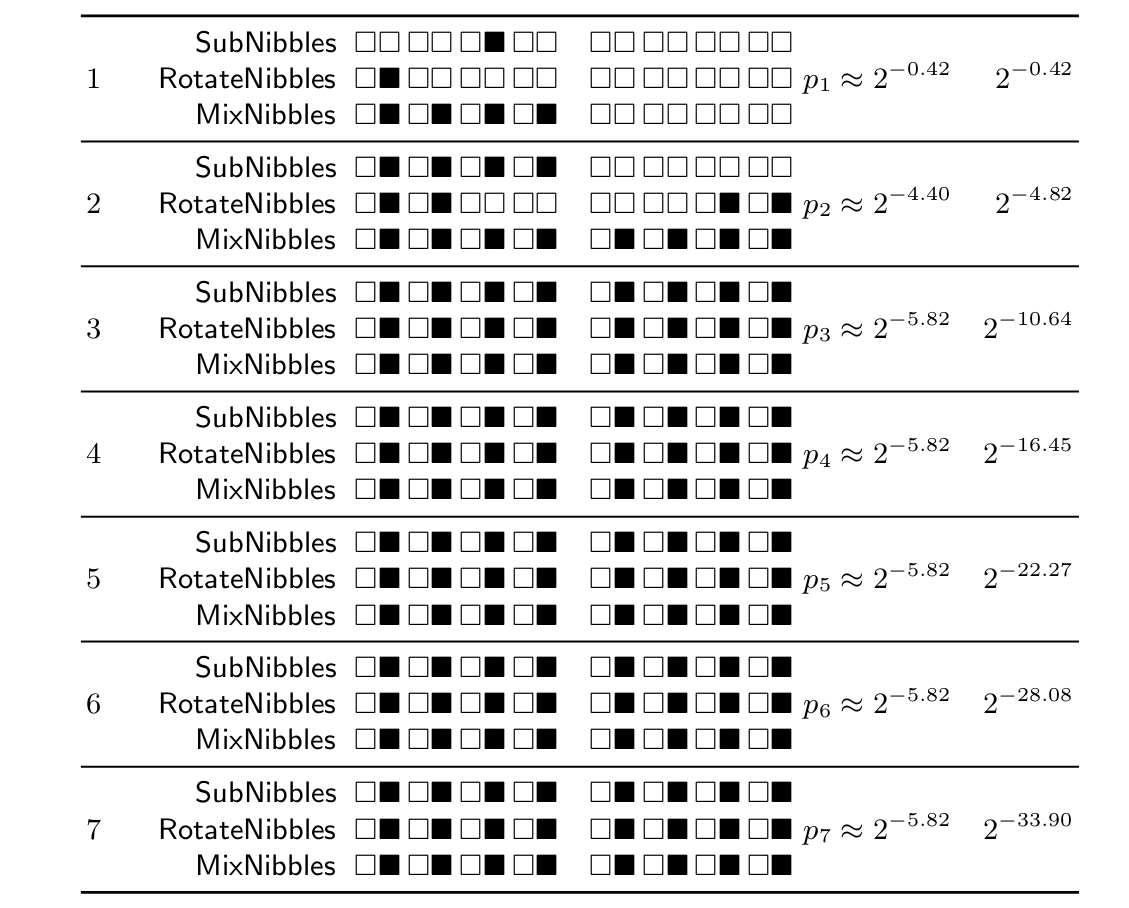
\includegraphics[width= \textwidth]{images/Representationcollectiondifferentialcharacteristics.png} 
    \caption{Representation of the collection of differential characteristics\cite{8round}}
    \label{fig:6distinguisher}
\end{figure}

\subsection{Attack on 8 Rounds of KLEIN}

\subsubsection{Finding and Exploiting Neutral Bits}
Lets start with defining a neutral bit, it is a bit wrt a given differential, ie flipping the bit in input conforming to the differential leads to new input conforming the same differential.The use of the  neutral bits is to decrease the time in searching and finding values conforming to differential.
The Input of a cryptographic function contains neutral bit.In plaintext block of the KLIEN we found that both the starting two and ending two bytes of input are neutral wrt to the collection of characteristics of the first two rounds.\\

The bytes first sent into the Sbox In first round, then after RotateNibbles they form the 4-byte 1/2 of the state which is as-well inactive in Mix-Nibbles.In the second round with out depending on the other bytes firstly our neutral bytes pass through the Sbox , the difference then they are mixed with remaining bytes within MixNibbles.output conformation of MixNibbles only depend on active nibbles, our bytes remain neutral un-till here, in the third round, values which enter Sbox depend on first and last two input bytes hence these are not neutral for third round.Hence having a given pair of inputs fulfilling the truncated differential, $2^{32}$ pairs conforming to first two rounds can be obtained by varying the first two and last two input bytes.\\

\subsubsection{Distinguisher for 7 Rounds}
According to the basis of 6-round differential characteristic a distinguisher for 7-round KLEIN-64 is constructed. The main point to examine here is that for a pair conforming to 6-round differential leads to all higher nibbles of the SubNibbles of round 7 being inactive.Because of the linearity property of the MixNibbles, we can find out the differences with only the output after 7 rounds inspite overcoming the effect of arbitary activation of nibbles due to MixNibbles after round 7.We can also tell that only lower nibbles active after SubNibbles.After $2^{28}$ observations, A conforming pair is likely to be detected where as In the Ideal case it should be $2^{32}$, which constitute the distinguisher. The distinguisher is slightly powerful: once a conforming pair is found in $2^{28}$, nearly 8 other pairs can be produced with negligible cost.\\


\subsubsection{Distinguisher for 8 Rounds}
The distinguisher for 7 Lead to finding one (and possibly many) conforming pairs at a lower cost than for an ideal cipher. For 8 rounds, the distinguisher consists in finding several pairs (rather than one) with reduced complexity. Firstly, one collects approximately $2^{33.90}$ pairs, and records the ones that conform to the output difference.Approximately 4 pairs satisfying the difference by chance are record , and one conforming to the collection of characteristics.It is observed that the conforming pair can be identified using the neutral bits. It follows that by testing $2^{32}$ derived pairs for each of the 5 pairs obtained initially, one new conforming pair is expected for the pairs obtained by chance and about 8 new pairs for the one conforming to the characteristics.Therefore, with about $2^{33.90}$ + 4 × $2^{32}$ ≈ $2^{35}$, one expects to find twice more conforming pairs than ideally.\\

\subsubsection{Key-Recovery for 8 Rounds}
The 7 rounds key-recovery attack can be derived by using the distinguisher of 4.1.2 for
finding the pair satisfying the 6-round differential.We exploit the invertibility of final MixNibbles and RotateNibbles to find-out output differences of every nibble after final SubNibbles.Further, the attack tries values of lower nibbles the linear combinations of key bits send them through Sbox; the difference thqat we get is then inverted after MixColumn; if difference only has lower nibbles active, then this is a possible guess.Given lower only active nibble the inverse MixNibbles result in lower only active nibbles with probability $2^{−3}$, The Search space is thus compacted from $2^{16}$
to $2^{13}$ for each of the two MixColumn instances.Further, total cost of key-recovery gets reduced to $2^{58}$ trials. The attack always be fruitful because we are trying all candidate keys in the $2^{58}$ trials.This is improved further using several conforming pairs. Using neutral
bits, one can produce 8 more pairs in $2^27$ where only 6 of them are enough to
find out the right combination of key bits, by taking intersection of $2^{13}$ element sets for each conforming pair.We reobtain the 32 bits which correspond to the XOR of lower nibbles of ciphertexts.Linear combination of the key bits will result in further expansion and reaches almost equivalent to recovering 32 key bits. The remaining 32 key bits are bruteforced in $2^32$.The attack thus recovers the 64-bit key with less than than $2^{33}$ encryptions.\\

if we extend the strategy of the 7-round attack to 8 rounds, mentioned as in 4.1.3 to detect the conforming pairs leads to “false alarms” (i.e. values conforming to the input/output differential
but not necessarily to this context). Thus with less than $2^{34}$ encryptions, one thus can identify a high probability conforming pair.Using neutral bits, one expects to produce almost 8 other conforming pairs after $2^{32}$ trials which is more than enough to identify with certainty 32 bits
of the last subkey. Overall, the 64 bits of the last subkey can be found with complexity less than
$2^{35}$ encryptions.\\


\subsection{Side-Channel Attack on KLEIN}
KLEIN posses a highly balanced key schedule wrt its opposition against Key-Related attacks and the dexterity of the keys, secret sharing method for resistance of side-channel attacks.Introducing noise and loops is easy in software implementation of a block-cipher to prevent side-channel attacks,For securing the hardware implementation of KLEIN.We already know that as far as the SubNibbles step is considered KLEIN is completely linear. The S-box of KLEIN can be implemented to resist side-channel attacks even in the presence of glitches using the secret sharing method proposed which is based on multi-party-computation protocols.using The three main properties namely Correctness,Uniformity and Non-Completeness.These help by computing the correlation between the average power consumption of device and the hypothetical power consumption with the help of a guessed key.The Linear part of KLEIN can be securely dealt-with by using independent shares.The masking based on secret sharing increases the hardware overhead, still promising because it was theoretically proven to be secure against DPA attacks. Differential power analysis is a side-channel attack involving mathematically analyzing power consumption measurements from a cryptosystem.\\

\subsection{Performance Evaluation On AVR microcontroller}

\subsubsection{With Respect To Energy Consumption}
To measure energy consumption, it is assumed that
the energy per CPU cycle is fixed.This energy consumption
includes the key scheduling and encryption.KLEIN is the best algorithm in comparison to other ciphers in aspect of energy consumption. We learnt many important factors that effect the energy consumption such as the performance of code depends on several specifications of a cipher such as
the Type of instructions, Mode of operation, Structure, Number of loops,Number of Rounds etc. Another important factor is which kind of instruction.it is important factor to use correct instruction
to write a code.\\

\begin{figure}
    \centering
    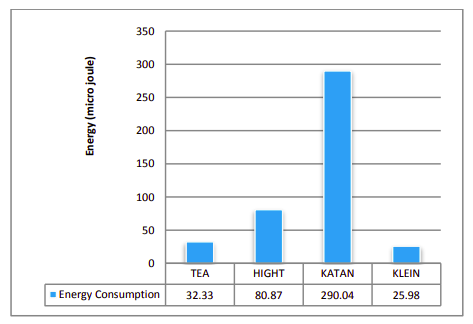
\includegraphics[width= 75 mm]{images/EC.png} 
    \caption{Energy consumption comparison of focused ciphers}
    \label{fig:6distinguisher}
\end{figure}

\subsubsection{With Respect To Memory Efficiency}

Few lightweight Cryptographic algorithms are analyzed in this part and there Similarities and Differencies With KLEIN. The memory usage of various lightweight algorithms is compared in
Figure 5 which shows the percentage of memory used for each cipher. Analyzed results clearly state that  KLEIN uses longer Flash memory space than the rest because the assembly code size of this algorithm is more than others Where as the percentage of SRAM usage for KLEIN cipher is not high as other ciphers. The Data Memory Usage for KATAN and KLEIN algorithm is equivalent\\

\begin{figure}
    \centering
    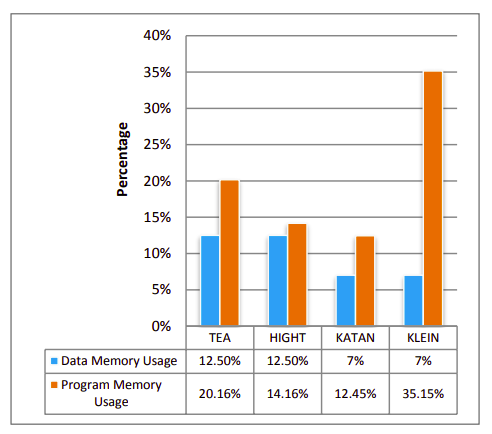
\includegraphics[width= 75 mm]{images/DM.png} 
    \caption{Data and Memory Usage of focused ciphers}
    \label{fig:6distinguisher}
\end{figure}

\subsubsection{With Respect To Security}
Taking degree of confusion and diffusion as the security criteria. KLEIN has least degree of diffusion
highest degree of confusion.This is related to the fact that of different structure.KLEIN is SPN and others  Feistel.


\section{Conclusion}
In this paper,We have described the Design Specifications of KLEIN Cipher, Different attacks on KLEIN Cipher,Performance of KLEIN is Compared with other lightweight Ciphers.The goal is to explain how KLEIN is the practical and secure cipher for low-resource applications.Hardware efficiency of KLEIN from its simple structure with an involutive S-box. If we further modify rotate nibbles algorithm and Increase diffusion we can prevent the above described attacks.\\


% \label{sec:main}
\printbibliography
%%%% 8. BILBIOGRAPHY %%%%

%%%% NOTES
% - Download abbrev3.bib and crypto.bib from https://cryptobib.di.ens.fr/
% - Use bilbio.bib for additional references not in the cryptobib database.
%   If possible, take them from DBLP.


\end{document}
